\section{Innovations}

\subsection{Updating the Expert System}
In academia and industry the term expert system has lost its luster.
Expert systems ended up only seeming like experts to those with the vocabulary for the task for which it was designed.
AI researchers, before the age of ubiquitous deep learning, almost all have experience designing and building expert systems of one type or another, giving us insight on the strengths and weaknesses of these types of systems.
The main weaknesses of expert systems, before the age of \gpts, and latter, type \llms\  and powerful generative AI (\gai), are the inclusion of new information (data ingestion) and the ability to make smart inferences on all knowledge available to it.
\llms\ have an uncanny knack for information ingestion and inference; however, due to the way neural networks learn information perfect inference is not a possibility.
Because perfect inference is not possible even when deduced by models with billions of parameters, the expert system must guide the output of the model by querying a knowledge base of data on which the system is to be an expert.
\llms\ allow the interface to the expert system to be accessible by anyone who can speak a language that it can understand.
\llms\ understand natural language and can perform high-level inference in response to natural language making them an extremely important component of an evolved expert system.
An expert system requires an inference engine and a knowledge base.
Modern LLms provide the inference engine, while the knowledge based can be curated, and finally the process must be moderated such that LLM hallucination can not interfere with the results; because what use is an expert system that will not tell you the truth?

Software oracles are the different experts to whom you can ask questions in an expert system.
The system as it exists only relies on the documents on which it is trained to answer questions; however, being confined to just this is not close to being suitable for our use case.
Our use case being a system that is an overall expert concerning genetic and genomics research on rats and mice in the \GN\ database and ecosystem.
The experts in this research area have access to and knowledge of more than the documents that pertain to \GN\ but many scientific texts, publishing houses, knowledge bases and more.
For example, the Bing chat system uses wikipedia, a large online encyclopedia, and many online scientific sources.
The scientists that operate and maintain \GN\ have created metadata reference information, and other data points that can be added to the system and will create more of an oracle of the LLM trained system.
While other resources, line PubMed, have its own APIs so it is an open oracle that can be queried to support the \project.
%\subsection{Not Just Machine Learning (ML)}

A system should be built that supports researchers of varying levels of ability.
This system should be able to communicate well with people with differing levels of knowledge who seek variable levels of atomicity.
On the scale of accommodating people with differing levels of knowledge, Bing chat, co-developed by OpenAI and Microsoft, performs admirably.
When querying the system about a specific transcription factor, it not only provides a summarized description of the subject, but also returns citations as links.

%\newpage
%\captionsetup{font={scriptsize,sc,up,singlespacing}}
\begin{figure}[h] % Figure at bottom of the page ([b] argument, could be "t" for top or "h" for here)
	\centering
	%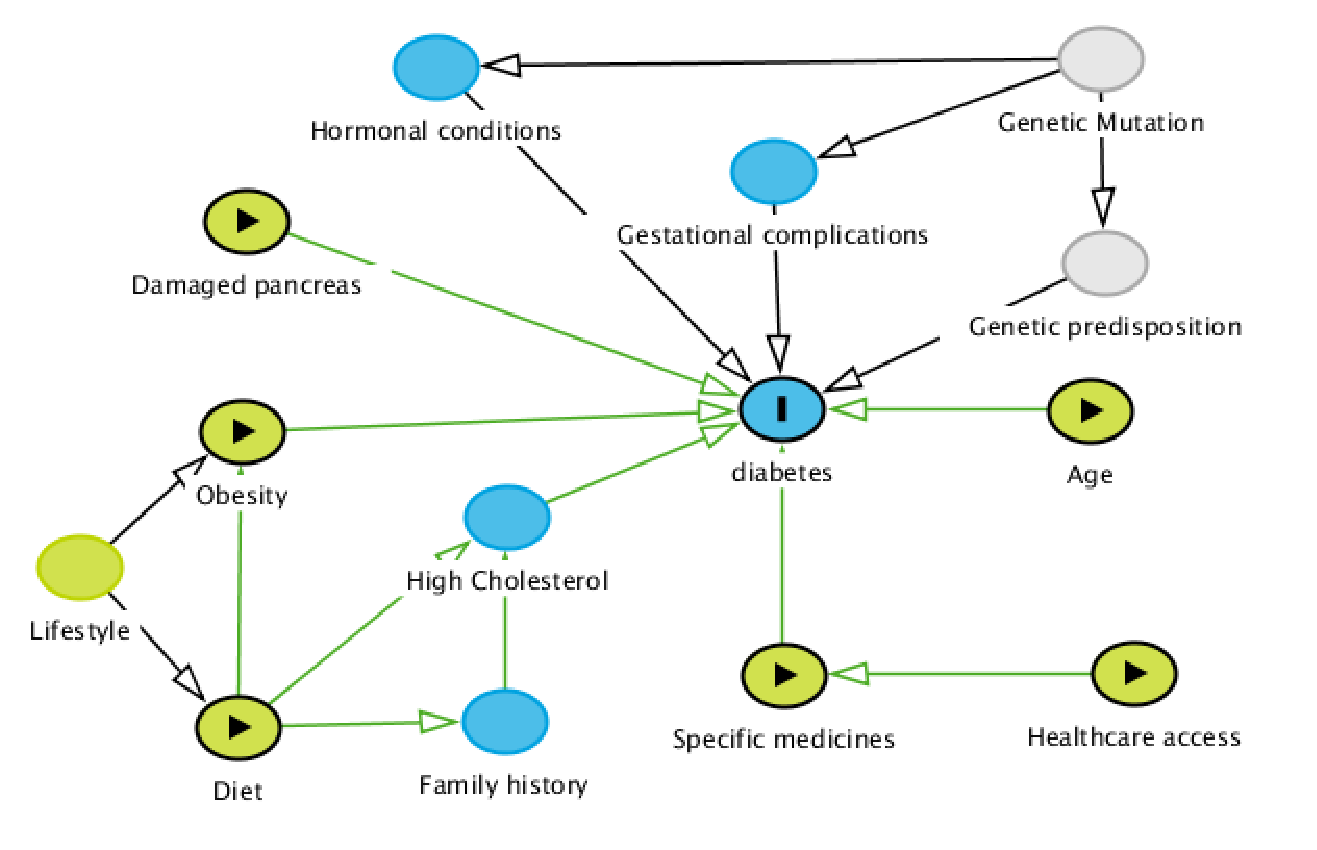
\includegraphics[width=\textwidth]{diabetes-causalmodel.eps}
	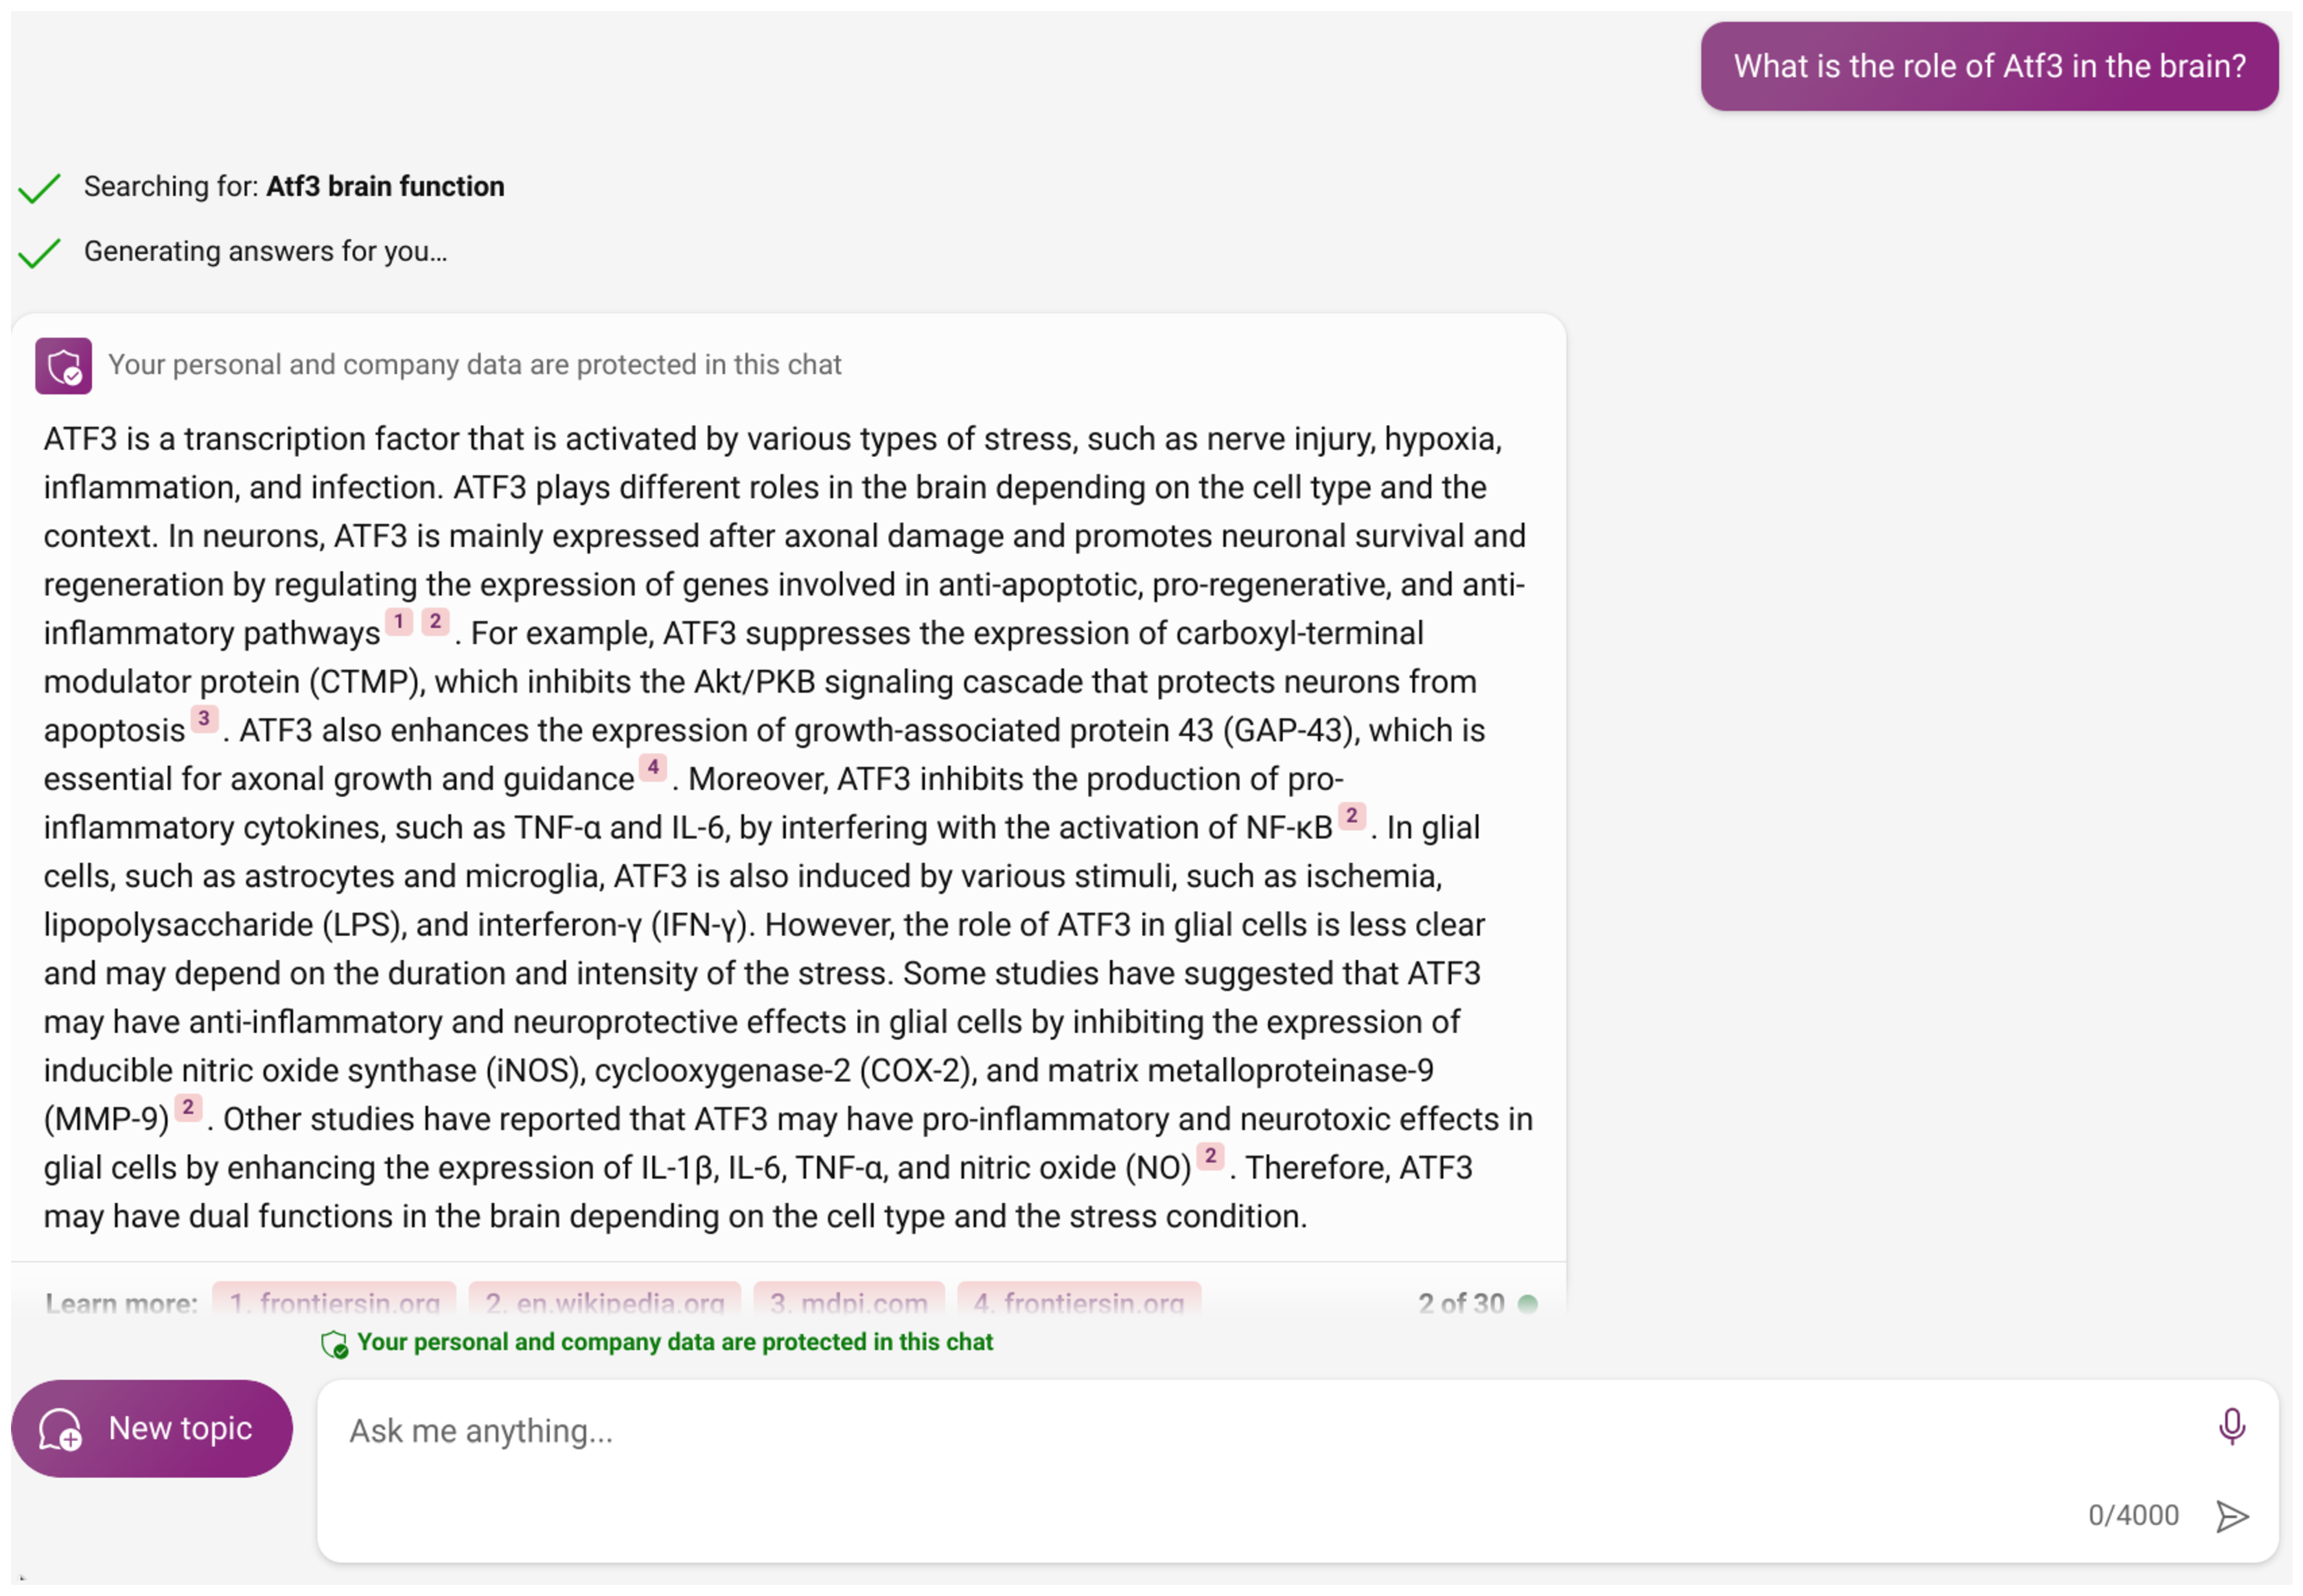
\includegraphics[width=.5\textwidth]{bingchat_atf3.eps}
	\caption{ \textbf{Bing Chat Query and Answer Example}
    The same question was asked BingChat and the existing demo of GNQA: `What is the role of Atf3 in the brain?'. 
            }
        \label{fig:atf3-chatcomparison}
\end{figure}


Bing's chat interface combines with it search, making it similar to what we have envisioned. 
Bing is using its search as an Oracle as when asked biological questions it returns answers from wikipedia.org and popular scientific publishing houses, as can been seen in figure~\ref{fig:atf3-chatcomparison}.
We want the GeneNetwork Question and Answer system to work similarly where search and summarization are handled and combined in a response.
The current version of our question answering system returns multiple references with each response, and will later return links to papers in PubMed and other refernce sites, along with links to datasets when sensible.

%\newpage
%\captionsetup{font={scriptsize,sc,up,singlespacing}}
\begin{figure}[h] % Figure at bottom of the page ([b] argument, could be "t" for top or "h" for here)
	\centering
	%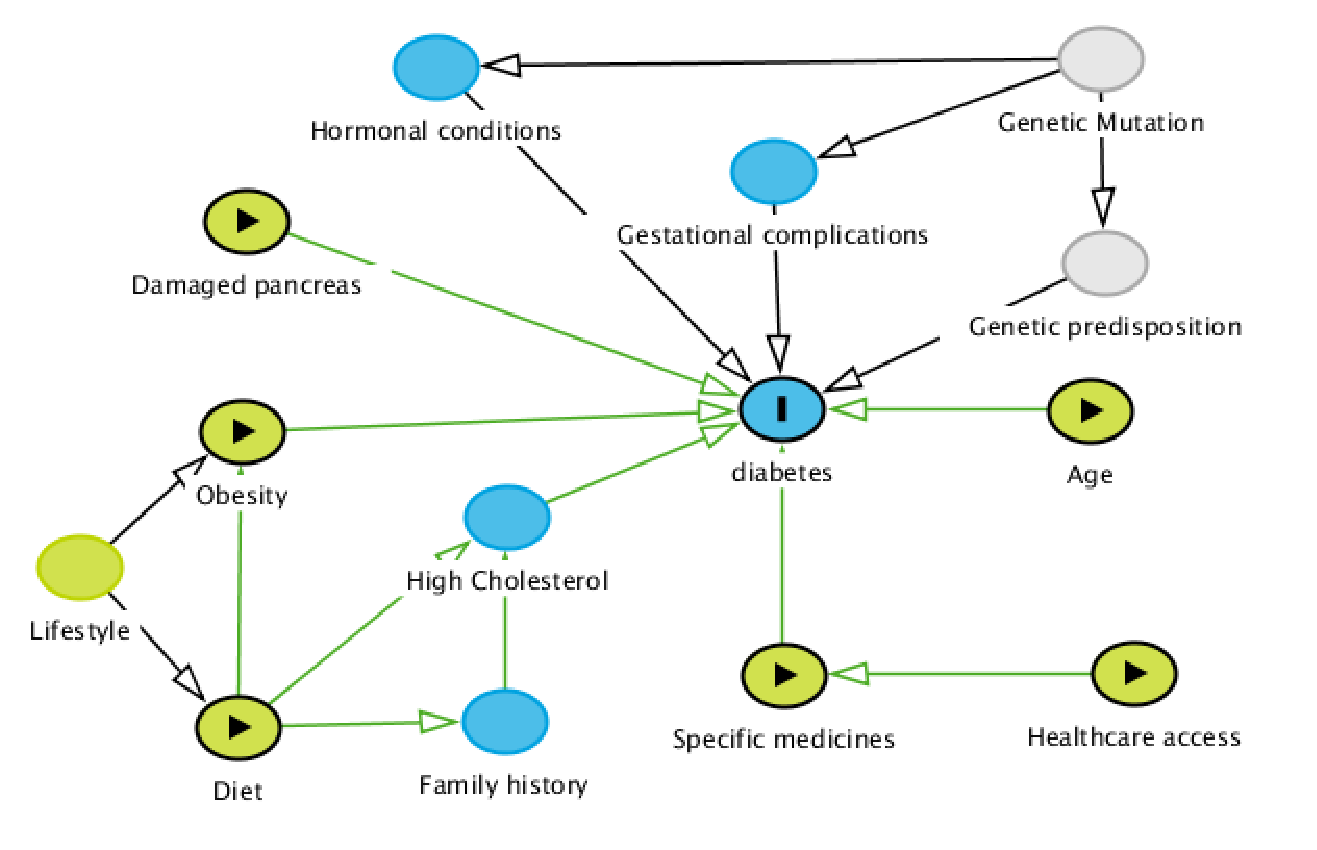
\includegraphics[width=\textwidth]{diabetes-causalmodel.eps}
	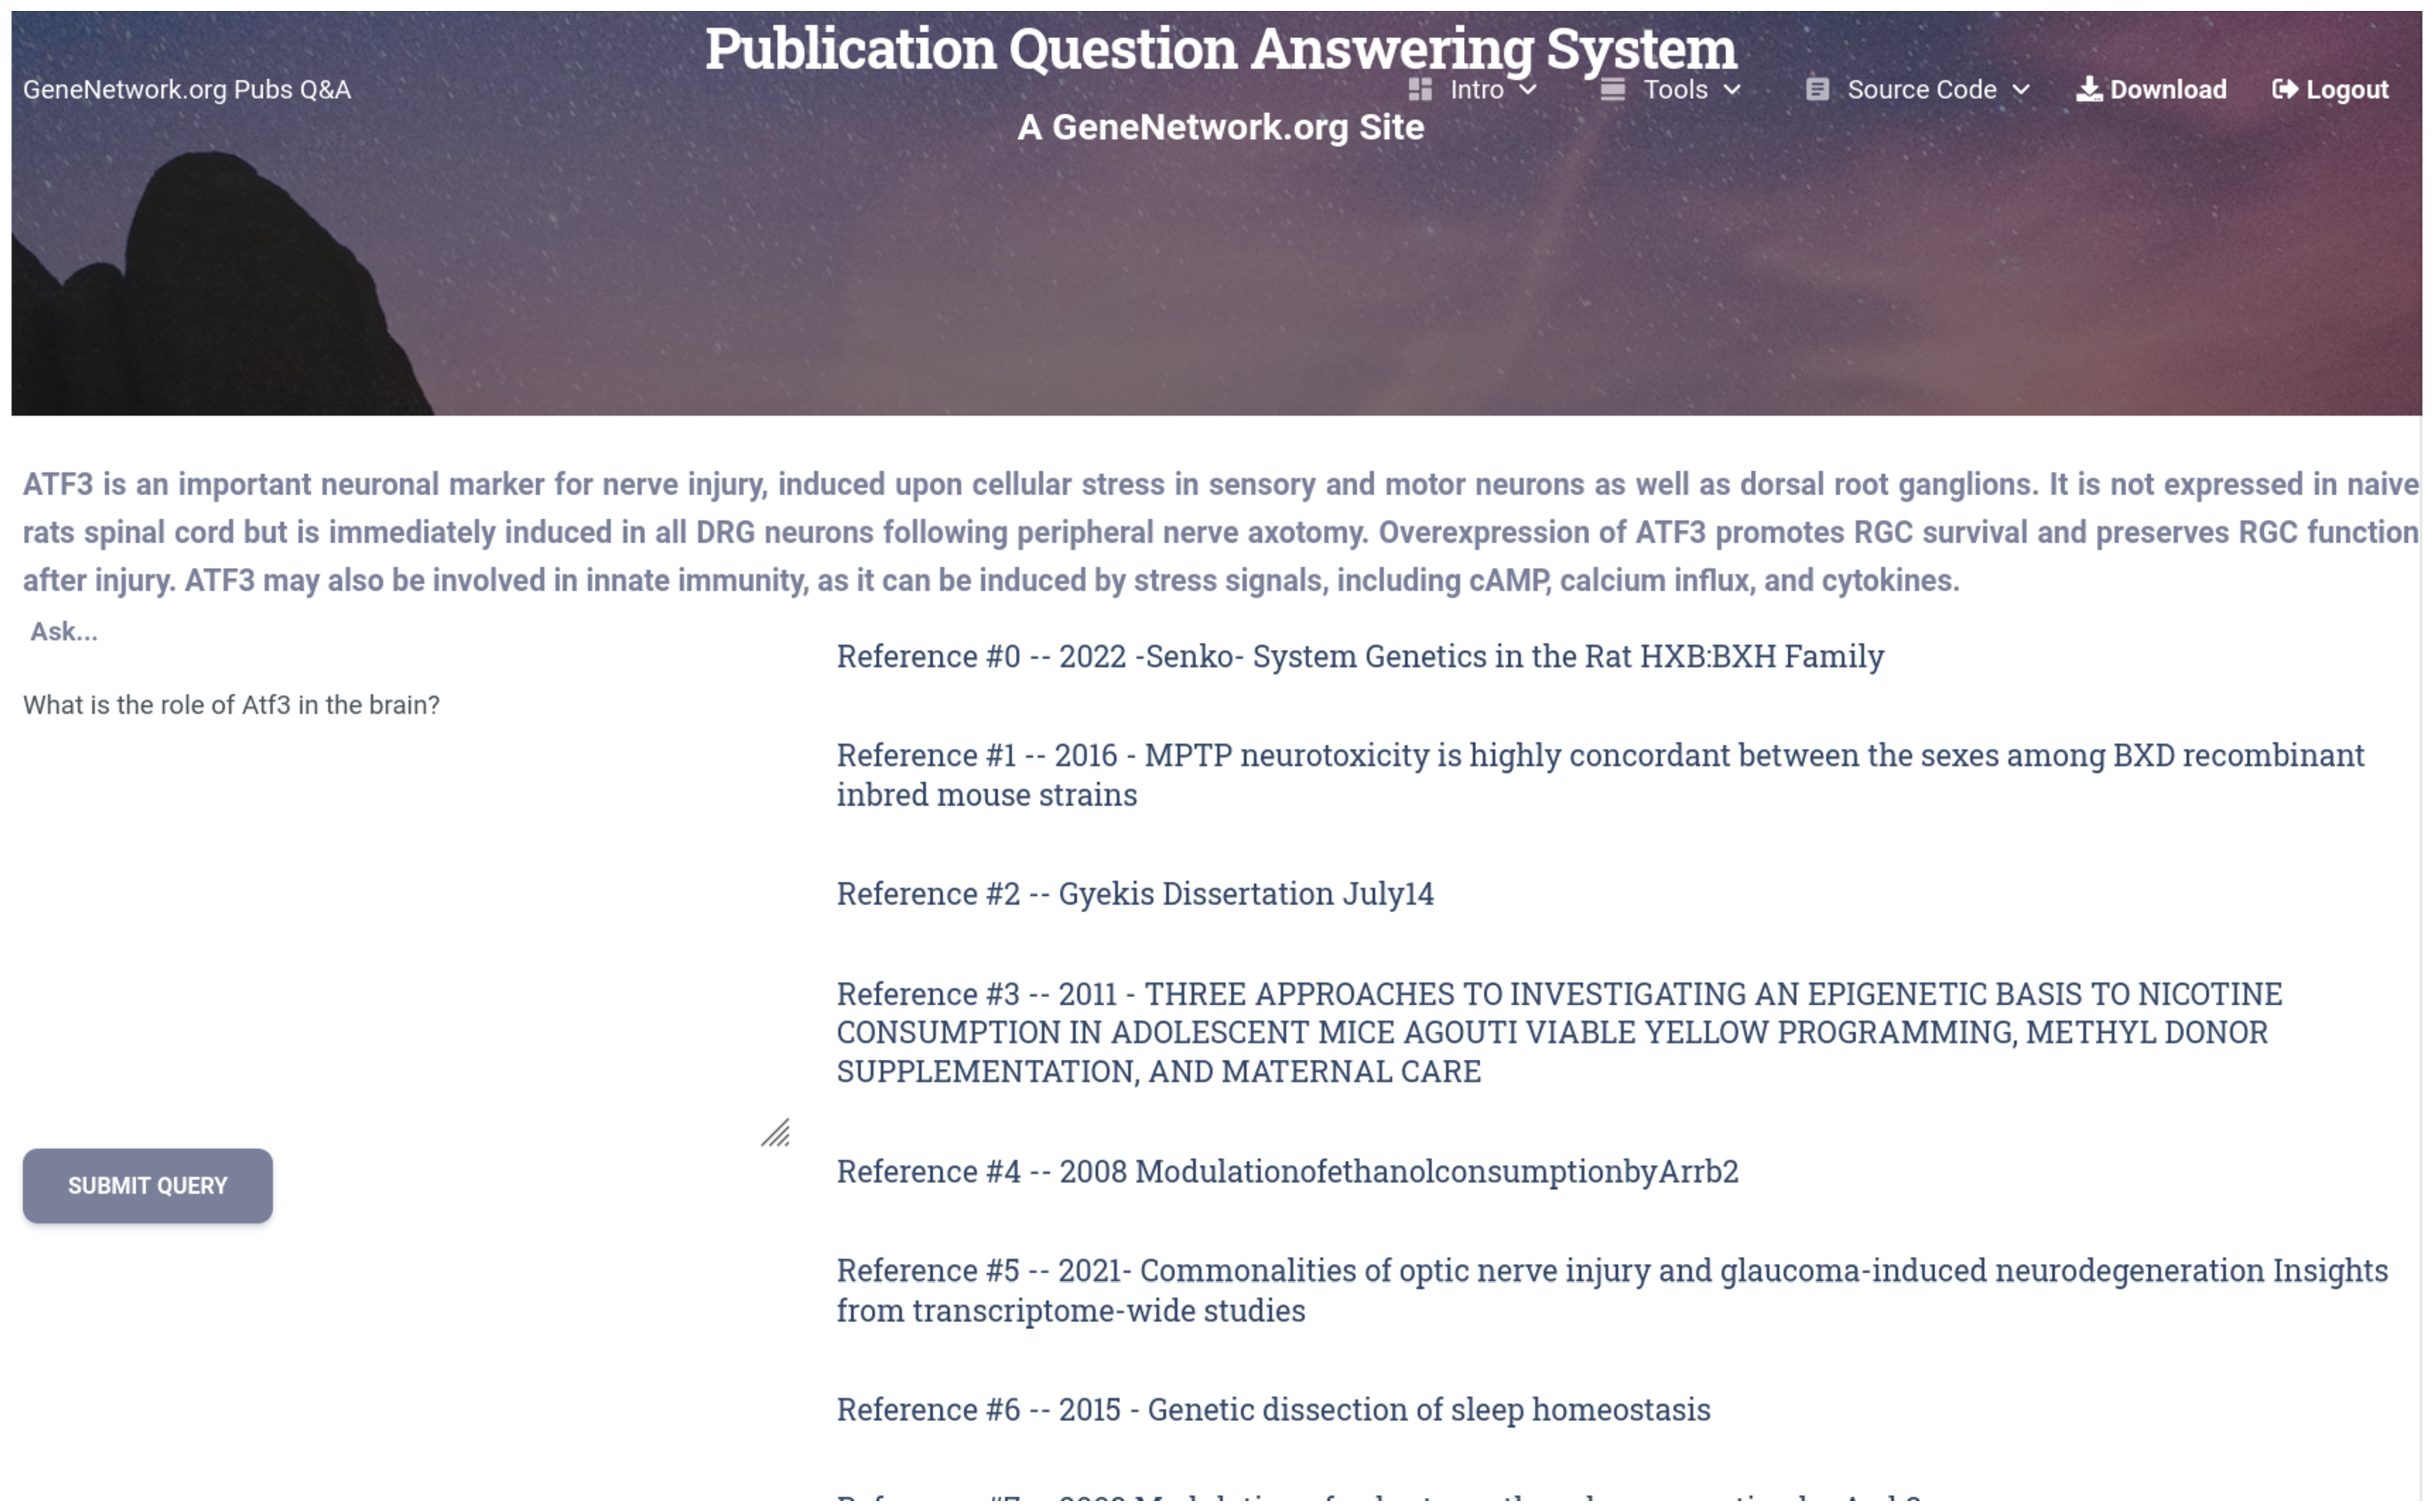
\includegraphics[width=.5\textwidth]{gnqa_atf.eps}
	\caption{ \textbf{GeneNetwork.org Query and Answer Example}
    The same question was asked BingChat and the existing demo of GNQA: `What is the role of Atf3 in the brain?'. 
            }
        \label{fig:gnqa_atf}
\end{figure}


Looking at figure~\ref{fig:gnqa-atf3-qa} one can see that references are returned with summaries for immediate further reading.
The systems development will later include links to other sites with scientific works and datasets on which studies and experiments have been conducted, from the publications of interest that have used the \GN\ database.
Our system is meant to be a support tool for researchers while being a tool that can help a novice or citizen scientist learn more about \GN\ research.